\begin{tips}
    直线只研究方向向量，平面只研究法向量。
\end{tips}

\begin{theorem}[叉乘法求法向量]
    设 $\overrightarrow{A B}, \overrightarrow{A C}$ 是平面 $A B C$ 的两个不共线的向量，则平面 $A B C$ 的法向量可以用叉乘法。

    具体的操作是：求谁盖谁，Y 加负号。
\end{theorem}

\section{异面直线所成的角}

\subsection{通过平移与余弦定理构造}

\begin{example}
    已知长方体 $A B C D-A_1 B_1 C_1 D_1, A B=2, A D=1, A A_1=\sqrt{3}$ ，则直线 $A_1 B$ 与直线 $B_1 C$ 所成角的余弦值为 （\qquad）
    \begin{tasks}(4)
        \task $\frac{3 \sqrt{7}}{7}$
        \task $\frac{3 \sqrt{7}}{14}$
        \task $\frac{2 \sqrt{7}}{7}$
        \task $\frac{\sqrt{14}}{7}$
    \end{tasks}
\end{example}

\begin{figure} [H]
    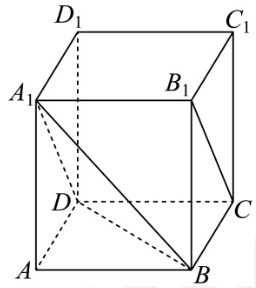
\includegraphics[width=0.16\textwidth]{chapters/立体几何/images/建系法求角/img-20250824210822.png}
\end{figure}

\begin{example}
    如图所示，在正三棱柱 $A B C-A_1 B_1 C_1$ 中，$A A_1=A B=2$ ，则异面直线 $A_1 C$ 与 $A B_1$ 所成角的余弦值为 （\qquad）
    \begin{tasks}(4)
        \task $\frac{1}{2}$
        \task $\frac{\sqrt{2}}{2}$
        \task $\frac{1}{4}$
        \task $\frac{\sqrt{2}}{4}$
    \end{tasks}
\end{example}

\begin{figure} [H]
    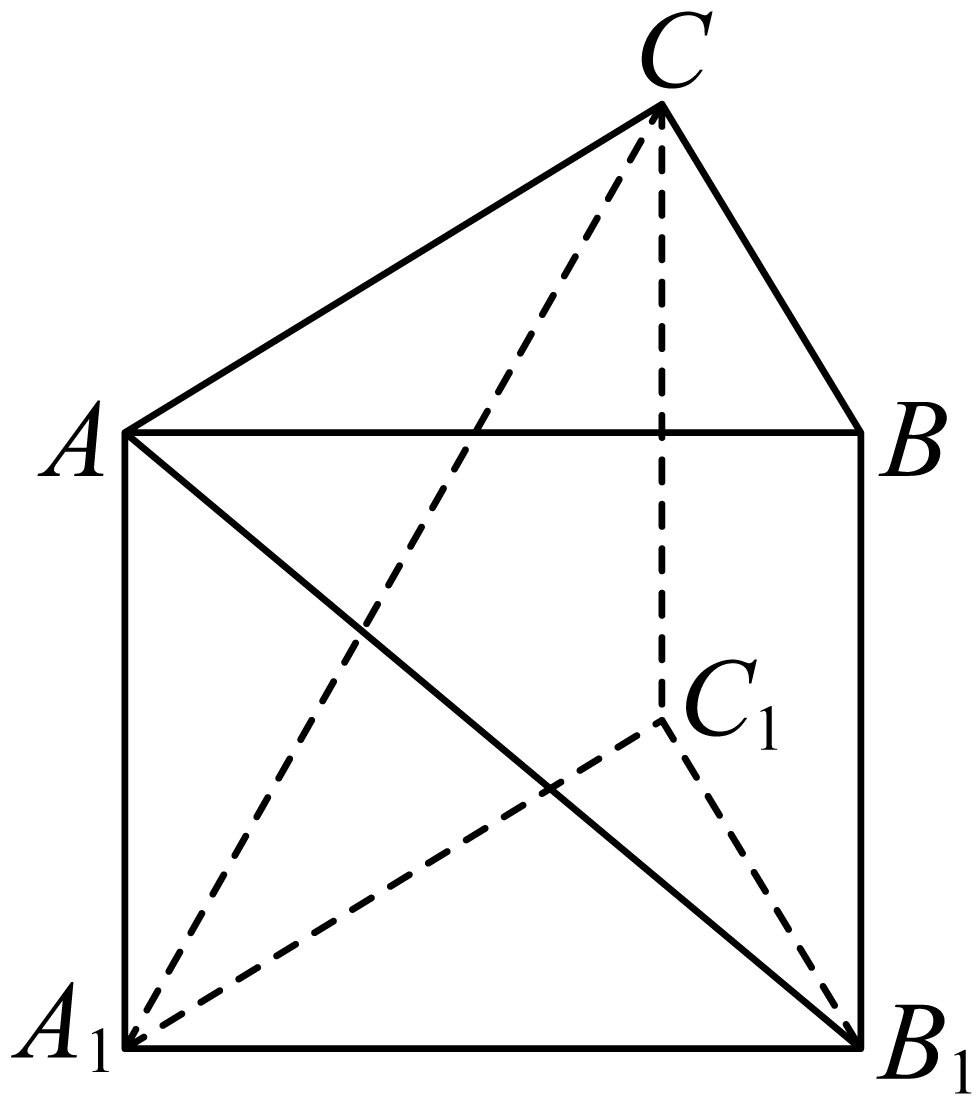
\includegraphics[width=0.16\textwidth]{chapters/立体几何/images/建系法求角/img-20250824211002.png}
\end{figure}

\subsection{通过建系求解}

\begin{example}
    正四棱锥 $S-A B C D$ 中，$O$ 为顶点 $S$ 在底面 $A B C D$ 内的正投影，$P$ 为侧棱 $S D$ 的中点，且 $S O=O D=\sqrt{2}$ ，则异面直线 $P C$ 与 $B D$ 的距离为 （\qquad）
    \begin{tasks}(4)
        \task $\frac{\sqrt{10}}{10}$
        \task $\frac{\sqrt{10}}{5}$
        \task $\frac{\sqrt{5}}{10}$
        \task $\frac{\sqrt{5}}{5}$
    \end{tasks}
\end{example}

\begin{figure} [H]
    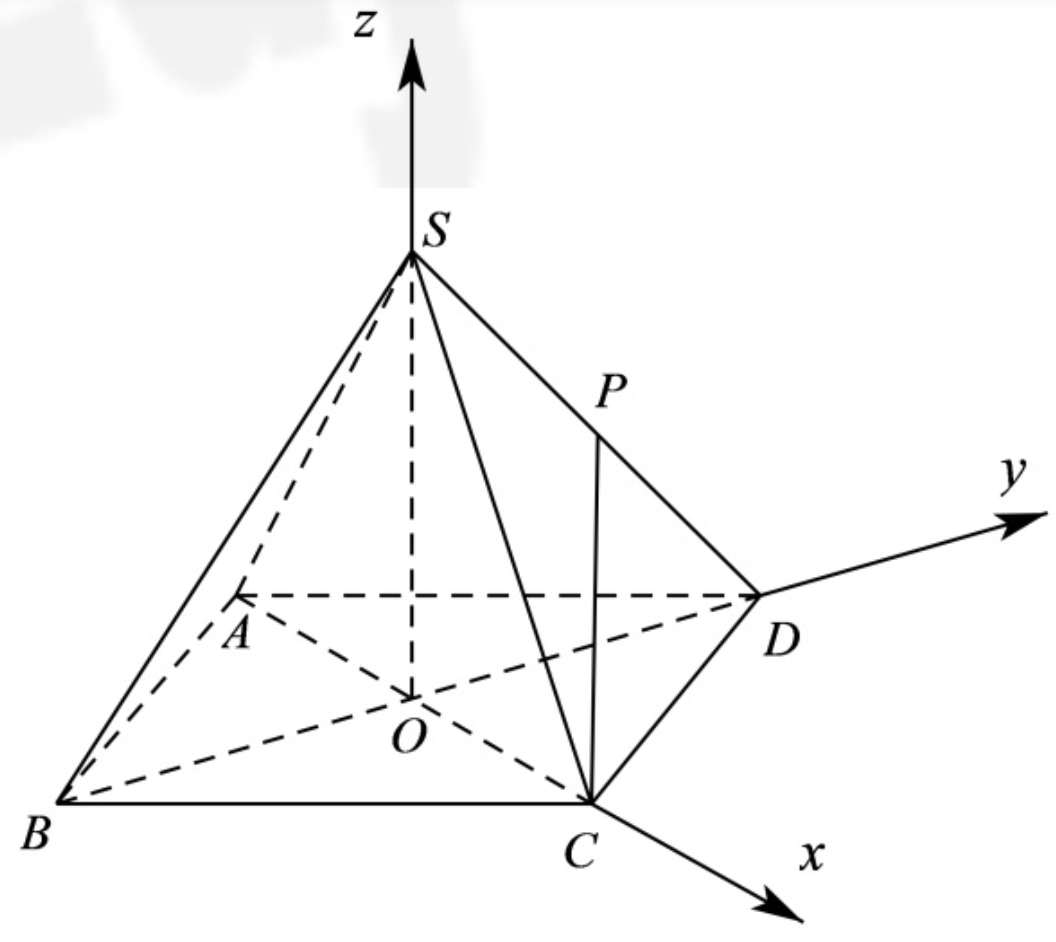
\includegraphics[width=0.25\textwidth]{chapters/立体几何/images/建系法求角/img-20250824211141.png}
\end{figure}

\begin{example}
    如图，四棱雉 $P-A B C D$ 中，$P D \perp D A, P D \perp D C$ ，在底面 $A B C D$ 中，$A B \| D C, ~ A B \perp A D$ ，且 $2 A B=C D=6, ~ A D=P D=4, ~ E$ 为 $P C$ 的中点．
    \begin{enumerate}
        \item 求证：$B E / /$ 平面 $A D P$ ；
        \item 求异面直线 $P A$ 与 $B C$ 所成的角的余弦值．
    \end{enumerate}
\end{example}

\begin{figure} [H]
    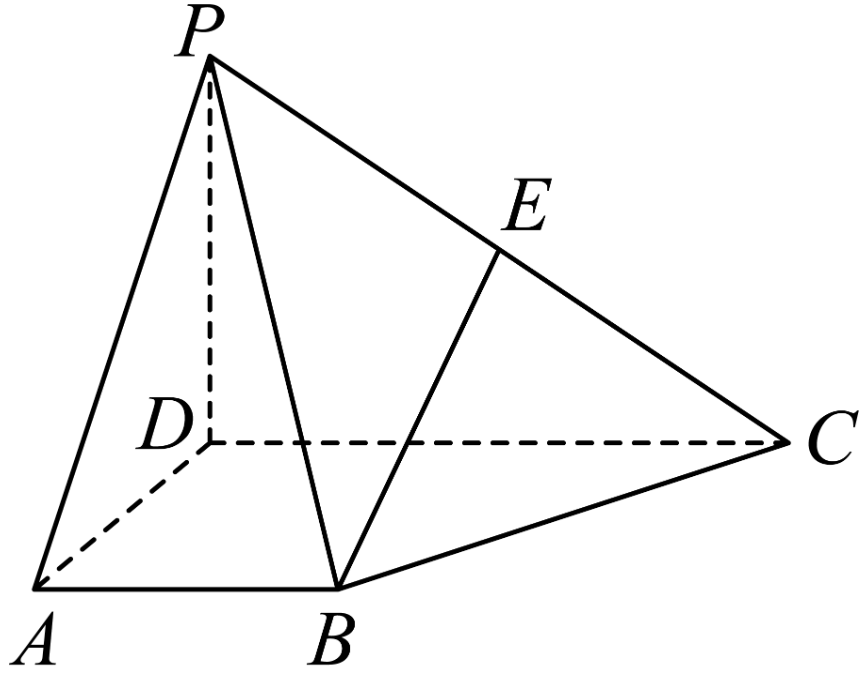
\includegraphics[width=0.2\textwidth]{chapters/立体几何/images/立体几何的几何法证明/img-20250824213020.png}
\end{figure}

\subsection{面面角与二面角}

\begin{theorem}

\end{theorem}


\section{空间中的动点和距离问题}

\begin{problem}
如图，在三棱锥 $A-B C D$ 中，$\triangle A B C$ 是正三角形，平面 $A B C \perp$ 平面 $B C D, ~ B D \perp C D$ ，点 $E, ~ F$ 分别是 $B C, ~ D C$ 的中点．
\begin{enumerate}
    \item[(1)] 证明：平面 $A C D \perp$ 平面 $A E F$ ；
    \item[(2)] 若 $\angle B C D=60^{\circ}$ ，点 $G$ 是线段 $B D$ 上的动点，问：点 $G$ 运动到何处时，平面 $A E G$ 与平面 $A C D$ 所成的锐二面角最小．
\end{enumerate}

\begin{figure} [H]
    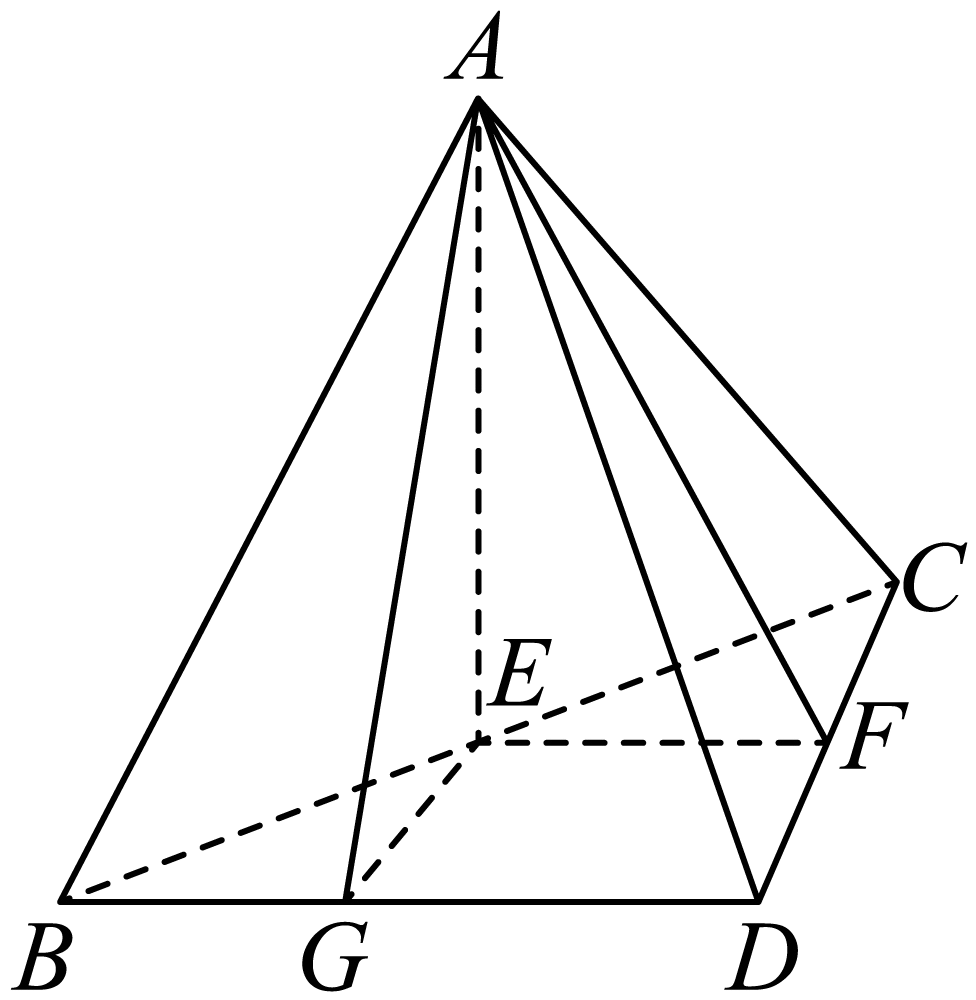
\includegraphics[width=0.2\textwidth]{chapters/立体几何/images/建系法求角/img-20250704221209.png}
\end{figure}

\end{problem}

\subsection{平面法向量与存在性问题}

\begin{problem}
如图，在四棱雉 $P-A B C D$ 中，$B D \perp P C, ~ \angle B A D=120^{\circ}$ ，四边形 $A B C D$ 是菱形，$P B=\sqrt{2} A B=\sqrt{2} P A, ~ E$ 是棱 $P D$ 上的动点，且 $\overrightarrow{P E}=\lambda \overrightarrow{P D}$.
\begin{enumerate}
    \item[(1)] 证明：$P A \perp$ 平面 $A B C D$ ；
    \item[(2)] 建立适当的空间直角坐标系，求面 $P A B$ 法向量和平面 $A C E$ 的法向量；
    \item[(3)] 是否存在实数 $\lambda$ ，使得平面 $P A B$ 与平面 $A C E$ 的夹角的余弦值是 $\frac{\sqrt{7}}{7}$ ？若存在，求出 $\lambda$ 的值；若不存在，请说明理由．
\end{enumerate}

\begin{figure} [H]
    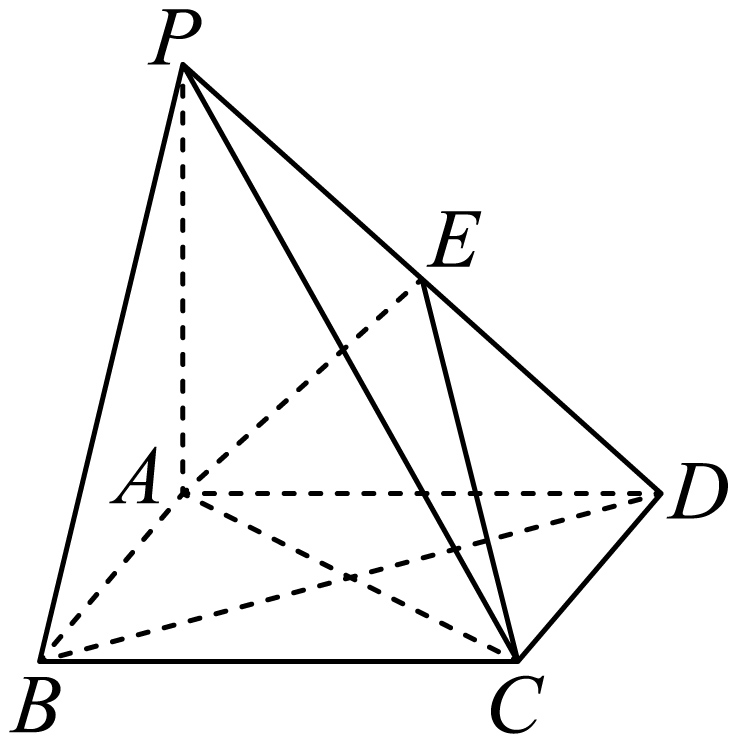
\includegraphics[width=0.2\textwidth]{chapters/立体几何/images/建系法求角/img-20250704221453.png}
\end{figure}
\end{problem}